\textit{Aleksandr Michajlovic Lyapunov} (1857-1918) proposed two methods to study the stability of a \textbf{non linear system}. The first is based on observations done on a \textbf{linearized system}, the second is based on seeking a particular function that could satisfy some properties.

\section{Linearization method (LM)}
It is often of interest to linearize a system either around an \textbf{equilibrium point} or a \textbf{trajectory}. Usually it is useful to analyze the system and control it in a proper way.\\
A non linear system has the form 
\begin{align*}
    &\dot{x(t)}=f[x(t), u(t)]\\
    &y(t)=h[x(t), u(t)]
\end{align*}
In this scenario we define the following quantities:
\begin{align*}
    &\delta x(t) = x(t)-\bar{x}\\
    &\delta u(t) = u(t)-\bar{u}\\
    &\delta y(t)=y(t)-h(\bar{x}, \bar{u})
\end{align*}

The \textbf{linearization step} is based on the \textbf{Taylor expansion} which states that \textbf{in the neighbourhood of an equilibrium point $x_0 $}, $$ f(x) = f(x_0)+\frac{\partial f}{\partial x} (x-x_0)$$
If we apply this result to the non linear system for both functions $f$ and $g$ we obtain: 
\begin{align*}
    \dot{x}= f(x,u) =\delta \dot{x}(t) &= 
        \frac{\partial f}{\partial x} \Bigg|_{(\bar{x}, \bar{u})} \delta x +
        \frac{\partial f}{\partial u} \Bigg|_{(\bar{x}, \bar{u})} \delta u\\
    \delta y(t) &= \frac{\partial h}{\partial x} \Bigg|_{(\bar{x}, \bar{u})} \delta x +
    \frac{\partial h}{\partial u} \Bigg|_{(\bar{x}, \bar{u})} \delta u
\end{align*}
Due to the fact that $f(x,u)$, $h(x,u)$ are \textbf{vector fields} the derivatives are \textbf{Jacobian matrices} which corrensponds to matrices $A, B, C, D$ of a linearized system
\begin{align*}
    &\delta \dot{x}(t)=A\delta x(t) + B \delta u(t)\\
    &\delta y(t) = C \delta x(t) + D \delta u(t)
\end{align*}
Where the matrices $A, B, C, D$ are defined as follows:
{
    \large{
        \begin{align*}
            &A = \begin{bmatrix}
                \frac{\partial f_1}{\partial x_1} & \ldots & \frac{\partial f_1}{\partial x_{n_x}} \\
                \vdots                            & \ddots &  \vdots \\
                \frac{\partial f_{x_n}}{\partial x_1} & \ldots & \frac{\partial f_{x_n}}{\partial x_{n_x}}
            \end{bmatrix}_{(\bar{x}, \bar{u})} \quad
            B = \begin{bmatrix}
                \frac{\partial f_1}{\partial u_1} & \ldots & \frac{\partial f_1}{\partial x_{n_u}} \\
                \vdots                            & \ddots &  \vdots \\
                \frac{\partial f_{x_n}}{\partial u_1} & \ldots & \frac{\partial f_{n_u}}{\partial x_{n_x}}
            \end{bmatrix}_{(\bar{x}, \bar{u})}\\
            &C = \begin{bmatrix}
                \frac{\partial f_1}{\partial x_1} & \ldots & \frac{\partial f_1}{\partial x_{n_x}} \\
                \vdots                            & \ddots &  \vdots \\
                \frac{\partial f_{x_n}}{\partial x_1} & \ldots & \frac{\partial f_{x_n}}{\partial x_{n_x}}
            \end{bmatrix}_{(\bar{x}, \bar{u})}  \quad
            D = \begin{bmatrix}
                \frac{\partial f_1}{\partial x_1} & \ldots & \frac{\partial f_1}{\partial x_{n_x}} \\
                \vdots                            & \ddots &  \vdots \\
                \frac{\partial f_{x_n}}{\partial x_1} & \ldots & \frac{\partial f_{x_n}}{\partial x_{n_x}}
            \end{bmatrix}_{(\bar{x}, \bar{u})}
        \end{align*}
    }
}
The \textbf{linearized system} represents an approximation of the non linear system in the neighbourhood of the equilibrium point $(\bar{x}, \bar{u})$
\subsection{Stability of an equilibrium point}
Let $\lambda_1, ..., \lambda_{n}$ be the eigenvalues of the $A$ matrix  previously defined. The \textbf{equilibrium point} $(\bar{x}, \bar{u})$ of the system is:
\begin{itemize}
    \item \textbf{Asimptotically stable} if and only if $\textrm{Re}(\lambda_i)<0 \quad \forall i$
    \item \textbf{Unstable} if exists an $i$ such that $\textrm{Re}(\lambda_i)>0$
    \item Nothing can be said in case of marginal stability of the linearized system. 
\end{itemize}

This method is very simple, but provide us a way to study only the \textbf{local stability}, moreover it does not give any information on stability when the linearized system is only \textbf{marginally stable}.

\section{Lyapunov Direct Method (DM)}
The \textbf{Direct Method (DM)} is not restricted to local motion. It gives a way to determine the stability properties by constructing an \textbf{energy-like function} called the \textbf{Lypunov Function}. The method is based on a \textit{physical observation}: \\

{
\Large{
\centering 
    If the \textbf{total energy} of a system is dissipated, then the  system must settle down to an \textbf{equilibrium point}. 
 }
}\\

For example if we analyze the \textbf{mass-spring-damper} system, we note that is impossible to find an analytical solution, moreover the \textbf{Linearization Method} does not give any useful information if the motion starts outside the linear range. Using instead the expression of \textbf{mechanical energy} we can find more useful information.\\
The \textbf{Lyapunov's Direct Method} is based on a generalization of this idea to more complex systems. Now it is the moment to formalize this concepts and give some useful definitions. \\

 %Per disegnare il box
\hspace*{-5mm}
\begin{tikzpicture}
\node [mybox] (box){%
    \begin{minipage}{.96\textwidth}     %Larghezza del box
            \noindent
\textbf{Definition (Positive definite functions)} A function $V: \mathbb{R}^n  \rightarrow \mathbb{R}$ is \textit{locally positive definite}, if for some ball $B_R=\{x: \lVert x \rVert \le R\}$, 
\begin{align*}
    &V(x)=0, \quad x=0\\
    &V(x)>0, \quad x\ne 0, x \in B_R
\end{align*}
If $B_R=\mathbb{R}^n$ then the function $V(x)$ is said to be \textbf{globally definite positive}.\\
    \end{minipage}
};
\end{tikzpicture}%



\begin{figure}[h]
    \centering
    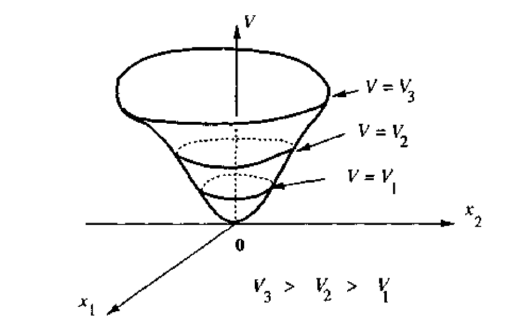
\includegraphics[scale=0.8]{NonLinearControl/images/PD_Fun.png}
    \caption{Example of a \textbf{Positive Definite Function}}
    \label{fig:enter-label}
\end{figure}

    %Per disegnare il box
\hspace*{-5mm}
\begin{tikzpicture}
\node [mybox] (box){%
    \begin{minipage}{.96\textwidth}     %Larghezza del box
            \noindent
\textbf{Definition (Positive semi-definite functions)} A function $V: \mathbb{R}^n  \rightarrow \mathbb{R}$ is \textit{positive semi-definite}, if for some ball $B_R=\{x: \lVert x \rVert \le R\}$, 
\begin{align*}
    &V(x)=0, \quad x=0\\
    &V(x)\ge0, \quad x\ne 0, x \in B_R
\end{align*}
    \end{minipage}
};
\end{tikzpicture}%

\vspace{0.5cm}

    %Per disegnare il box
\hspace*{-5mm}
\begin{tikzpicture}
\node [mybox] (box){%
    \begin{minipage}{.96\textwidth}     %Larghezza del box
            \noindent
\textbf{Definition} A function $V(x)$ is \textit{negative definite} if $-V$ is \textit{positive definite}. A function $V(x)$ is \textit{negative semidefinite} if $-V$ is \textit{positive semi-definite}. \\
    \end{minipage}
};
\end{tikzpicture}%



We are ready to give the definition of what is a \textbf{Lyapunov function}, two theorems based on the existence of such function can be used to recover the \textbf{stability properties} of a non linear system.\\

%Per disegnare il box
\hspace*{-5mm}
\begin{tikzpicture}
\node [mybox] (box){%
    \begin{minipage}{.96\textwidth}     %Larghezza del box
           \noindent
\textbf{Definition (Lyapunov function)} A functionm 
$V: \mathbb{R}^n \rightarrow \mathbb{R}$ is a \textit{Lyapunov function} if we can say that \textbf{for some ball} $B_R$, 
\begin{enumerate}
    \item $V(x)$ is positive definite and \textbf{has continuous partial derivatives},
    \item $\dot{V}(x)$ is negative semi-definite
\end{enumerate}

The derivative $\dot{V}(x)$ respect to time can be computed by using the \textbf{chain rule}: 
$$
    \dot{V}(x)= \frac{\partial V}{\partial x} \frac{\partial x}{\partial t} = 
    \nabla V(x) \dot{x} = \nabla V(x) f(x) 
$$
Using the fact that for an autonomous system we have $\dot{x}(t)=f(x)$
    \end{minipage}
};
\end{tikzpicture}%

\begin{figure}[h]
    \centering
    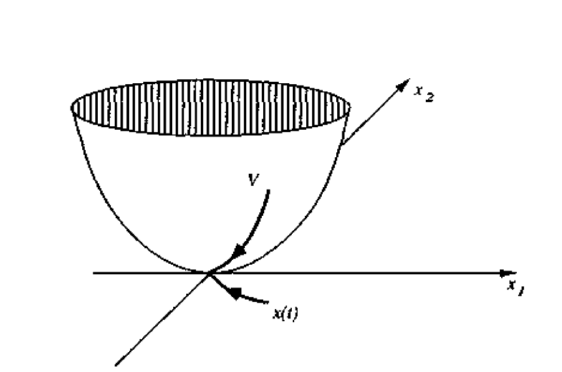
\includegraphics[scale=0.6]{NonLinearControl/images/LyapunovFunction.png}
    \caption{Example of a \textbf{Lyapunov Function}}
    \label{fig:enter-label}
\end{figure}

Without loss of generality we can assume that $\bar{x}=0$ is an equilibrium point, about the stability we have these theorems: \\


%Per disegnare il box
\hspace*{-5mm}
\begin{tikzpicture}
\node [mybox] (box){%
    \begin{minipage}{.96\textwidth}     %Larghezza del box
         \noindent
\textbf{Theorem (local stability)} If the system 
\begin{align*}
    &\dot{x}(t)=f[x(t), u(t)]\\
    &y(t)=h[x(t), u(t)]
\end{align*}
-admits a \textbf{Lyapunov Function} for some ball $B_R$, then the equilibrium point $\bar{x}=0$ is (marginally) stable). \\
-If moreover the function $\dot{V}(x)$ is \textbf{negative definite} in $B_R$ then the stability is  \textbf{asymptotic}.\\
    \end{minipage}
};
\end{tikzpicture}%\\
\vspace{0.5cm}

%Per disegnare il box
\hspace*{-5mm}
\begin{tikzpicture}
\node [mybox] (box){%
    \begin{minipage}{.96\textwidth}     %Larghezza del box
            \noindent
{\textbf{Theorem (global asymptotic stability)} }
If a system admits a Lyapunov function for $B_R=\mathbb{R}^n$ and \\
-$\dot{V}(x)$ is negative definite in $\mathbb{R}^n$\\
-$V(x)$ is \textbf{radially unbounded}, that is $\lVert x \rVert \rightarrow \infty 
\Rightarrow V(x) \rightarrow \infty
$\\
The equilibrium point $\bar{x}=0$ is \textbf{globally asysmptotically stable} for the system. 
    \end{minipage}
};
\end{tikzpicture}%


\noindent
Such theorems are not constructive,  in the sense that they do not tell us how to build a \textbf{Lyapunov function}, there are some methods that do not allow us to find in general the functions, but only in some cases. Some common methods are:
\begin{itemize}
    \item \textbf{Physical insight approach}, when it is possible to use physical observations a very powerful analysis can be conducted for these systems; 
    \item \textbf{Krasovskii's Method}, it gives \textbf{sufficient conditions} based on the Jacobian of the matrix $A$ of the linearized system. 
    \item \textbf{Variable Gradient Method} where a particular form for the gradient of the function $V(x)$ is assumed, then we compute the $V(x)$ by integrating such gradient.
\end{itemize}

\section {An Example: The pendulum}
In this section are shown an example of \textit{Lyapunov function} for the pendulum case, such function satisfies the properties in the theorem above mentioned. It is: 
\begin{equation*}
    V(x)=2(1-\cos(x_1))+\frac{x_2^2}{2}+\frac{(x_1+x_2)^2}{2}
\end{equation*}
In particular we observe that: 
\begin{enumerate}
    \item $V(x)$ is a Lyapunov Function in a certain ball $B_R$
    \begin{figure}[h]
    \centering
    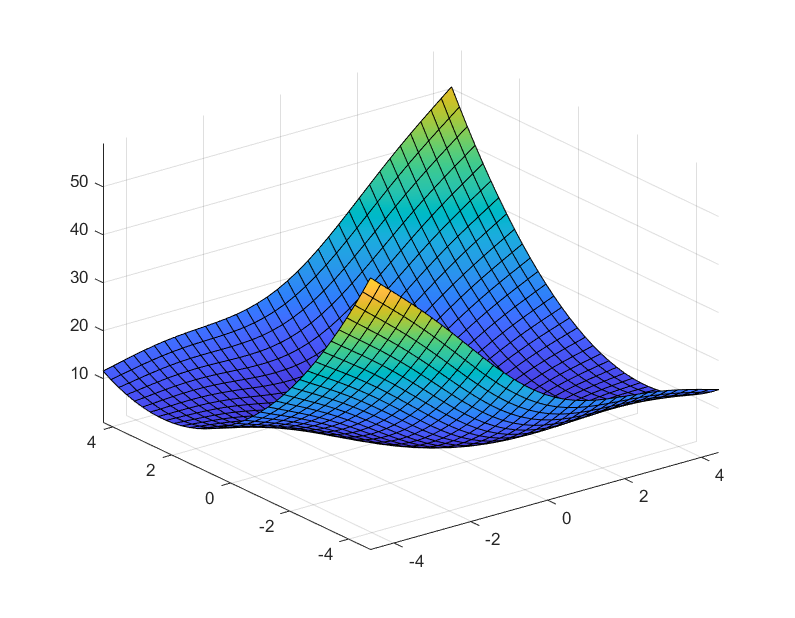
\includegraphics[scale=0.6]{NonLinearControl/images/Lyapunov.png}
    \caption{$2(1-\cos(x_1))+\frac{x_2^2}{2}+\frac{(x_1+x_2)^2}{2}$}
    \label{fig:enter-label}
    \end{figure}
    \item $\dot{V}(x)$ is \textbf{negative definite} in a certain ball $B_R$ centered in $\bar{x}=0$.  
\end{enumerate}

\begin{figure}[h]
    \centering
    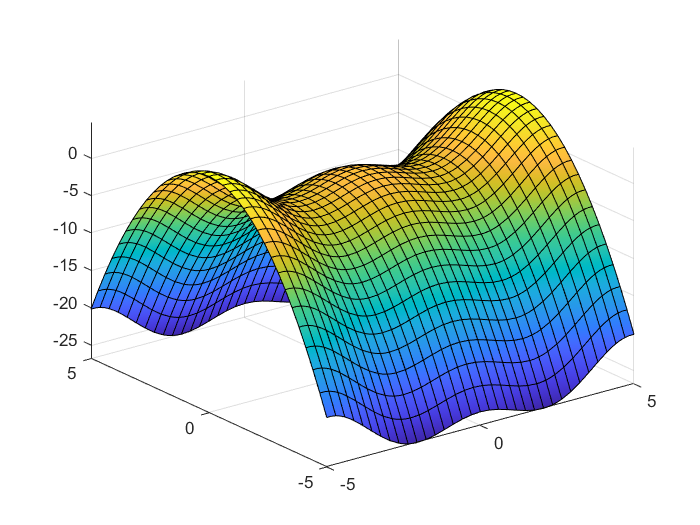
\includegraphics[scale=0.7]{NonLinearControl/images/Lyap_Der.png}
    \caption{$\dot{V}(x)$}
    \label{fig:enter-label}
\end{figure}
